%%
%% This is file `mcmthesis-demo.tex',
%% generated with the docstrip utility.
%%
%% The original source files were:
%%
%% mcmthesis.dtx  (with options: `demo')
%% !Mode:: "TeX:UTF-8"
%% -----------------------------------
%%
%% This is a generated file.
%%
%% Copyright (C)
%%     2010 -- 2015 by latexstudio
%%     2014 -- 2016 by Liam Huang
%%     2014 -- 2016 by latexstudio.net
%%
%% This work may be distributed and/or modified under the
%% conditions of the LaTeX Project Public License, either version 1.3
%% of this license or (at your option) any later version.
%% The latest version of this license is in
%%   http://www.latex-project.org/lppl.txt
%% and version 1.3 or later is part of all distributions of LaTeX
%% version 2005/12/01 or later.
%%
%% This work has the LPPL maintenance status `maintained'.
%%
%% The Current Maintainer of this work is Liam Huang.
%%
\documentclass{mcmthesis}
\mcmsetup{CTeX = false,   % 使用 CTeX 套装时,设置为 true
        tcn = 2010755, problem = A,% 队伍控制号码,接受一个字符串作为值;选题,接受一个字符串作为值;
        sheet = false, %为真时将输出摘要页,否则不输出;默认为 true。
        color = red,  %设置控制页的题目号的颜色
        titleinsheet = true, %为真时将在摘要页输出标题,否则不输出;默认为 false。
        keywordsinsheet = true,%为真时将在摘要页输出关键字,否则不输出;默认为 false。
        titlepage = false,%为真时将输出标题页,否则不输出;默认为 true。
        abstract = true}%为真时将在标题页输出摘要和关键词,否则不输出;默认值为 true。
\usepackage{palatino}  %控制正文字体,若是不喜欢可以注释掉。
\usepackage{lipsum}
\usepackage{tikz}
\usepackage{xcolor}
\usepackage{verbatim}
\usepackage{subfigure} 
\usetikzlibrary{arrows,shapes,chains}
\title{Title!}
\author{\url{http://www.latexstudio.net}\\[3pt]  \href{http://www.latexstudio.net/}
  {\includegraphics[width=7cm]{mcmthesis-logo}}}
\date{\today}

\makeatletter
\renewcommand*\l@section{\@dottedtocline{1}{12pt}{12pt}}
\makeatother

%%%%%%%%%%%%%%%%%%%%%%%%%%%%%%%%%%%%%%%%
%% MCM/ICM LaTeX Template %%
%% 2020 MCM/ICM           %%
%%%%%%%%%%%%%%%%%%%%%%%%%%%%%%%%%%%%%%%%
\usepackage{geometry}
\geometry{left=1in,right=0.75in,top=1in,bottom=1in}

%%%%%%%%%%%%%%%%%%%%%%%%%%%%%%%%%%%%%%%%
% Replace ABCDEF in the next line with your chosen problem
% and replace 1111111 with your Team Control Number
\newcommand{\Problem}{A}
\newcommand{\Team}{\# 2010755}
%%%%%%%%%%%%%%%%%%%%%%%%%%%%%%%%%%%%%%%%

\usepackage{newtxtext}
\usepackage{amsmath,amssymb,amsthm}
\usepackage{newtxmath} % must come after amsXXX

%\usepackage[pdftex]{graphicx}

\usepackage{fancyhdr}
\lhead{Team \Team}
\rhead{}
\cfoot{}

\newtheorem{theorem}{Theorem}
\newtheorem{corollary}[theorem]{Corollary}
\newtheorem{lemma}[theorem]{Lemma}
\newtheorem{definition}{Definition}

%%%%%%%%%%%%%%%%%%%%%%%%%%%%%%%%
\begin{document}
\graphicspath{{.}}  % Place your graphic files in the same directory as your main document
\DeclareGraphicsExtensions{.pdf, .jpg, .tif, .png}
\thispagestyle{empty}
\vspace*{-16ex}
\centerline{\begin{tabular}{*3{c}}
	\parbox[t]{0.3\linewidth}{\begin{center}\textbf{Problem Chosen}\\ \Large \textcolor{red}{\Problem}\end{center}}
	& \parbox[t]{0.3\linewidth}{\begin{center}\textbf{2020\\ MCM/ICM\\ Summary Sheet}\end{center}}
	& \parbox[t]{0.3\linewidth}{\begin{center}\textbf{Team Control Number}\\ \Large \textcolor{red}{\Team}\end{center}}	\\
	\hline
\end{tabular}}
\begin{Huge}
\begin{center}
\textbf{XXX}
\end{center}
\end{Huge}
%%%%%%%%%%% Begin Summary %%%%%%%%%%%
% Enter your summary here replacing the (red) text
% Replace the text from here ...
\begin{center}
\begin{large}
\textbf{Summary}
\end{large}
\end{center}



% to here
%%%%%%%%%%% End Summary %%%%%%%%%%%

%%%%%%%%%%%%%%%%%%%%%%%%%%%%%%
\clearpage
\pagestyle{fancy}

% Uncomment the next line to generate a Table of Contents
%\tableofcontents 

\setcounter{page}{1}
\rhead{Page \thepage\ of \pageref{LastPage}}
%%%%%%%%%%%%%%%%%%%%%%%%%%%%%%


\begin{abstract}
Firstly,\cite{1}

Secondly,

Thirdly,

We then

Finally,

\begin{keywords}
Generalized Additive Model, Markov model
\end{keywords}
\end{abstract}
\maketitle

\tableofcontents


\section{Introduction}




\section{Assumption}

There are some symbols appear in the model. We show them below:
\begin{table}[htbp]
\centering
\caption{Symbols in Chapter 3}
\begin{tabular}{cp{0.8\textwidth}}
\toprule
 Symbols & Description\\
\midrule
 $i$ & Station variable \\
\bottomrule
\end{tabular}
\end{table}

\section{M1}
------------- -------------  haven't decided where to put these sentences yet -------------  -----------------

We used LDA to get main topic of these reviews, and further draw a word cloud for each product. Word cloud is a direct way to demonstrate the frequency of words in a certain text. We show our word cloud of hair dryer as follows, other word clouds are attached to the appendix.Based on the rating level, we divide reviews into 2 categories: positive and negative. If the rating level is below 3, we regard words in this text as positive words and vice versa.\par
%word cloud of 1 product
\begin{figure}[htbp]
\centering
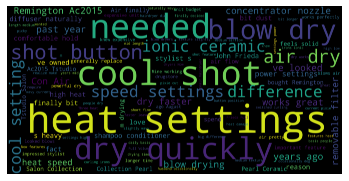
\includegraphics[width=10.5cm]{./figures/hairdryer_good.png}
\caption{Wordcloud (positive) of hairdryer}
\end{figure}
%wordcloud 
\begin{figure}[htbp]
\centering
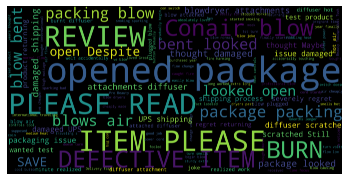
\includegraphics[width=10.5cm]{./figures/hairdryer_bad.png}
\caption{Wordcloud (negative) of hairdryer}
\end{figure}

From the word cloud we got, we found some important features that decides a product is popular is popular or not.
We list serval characteristic or points which are concluded from our word frequency research by classifying different rating levels separately.\par
%table
\begin{table}[htbp]
\centering
\caption{Keywords in reviews}
\begin{tabular}{cp{0.8\textwidth}}
\toprule
 Product Name & Description\\
\midrule
Hairdryer &Heat and speed settings, dry, package\\
Pacifier & Shape, smooth, quality, easy to clean\\
Microwave & Appliance, stainless material, mode and function\\
\bottomrule
\end{tabular}
\end{table}
As the table shows, customers have different requirements for different products. For example, hair dryer are reviewed most with words like heat settings, speed setting, how fast does the product dries, and its package. They complain for a terrible package.\par
For pacifier, parents expect them to be in suitable shape so that it fits well in a baby’s mouth. Besides, pacifier are judged according to their materials and whether it is easy to clean. If a pacifier is of low quality and without a cute shape, it will be rated with 1 star most likely.\par
For a microwave, most consumers want it to fit well in their kitchen and works well with a stainless appearance and multiple functional modes like grill mode, convection settings, heating settings.
And customers do not want microwaves stop working after a few weeks and thus require a good after-sale service.


------------- -------------  haven't decided where to put these sentences yet -------------  -----------------


\section{M2}

\section{M3}




\section{Strengths and Weaknesses}
\subsection{Strengths}



\subsection{Weaknesses}


\section{A Letter}
------------- -------------  part of letter -------------  -----------------\par
To whom it may concerns:\par

For sales of hair dryers, customer care more about its quality, for example, how fast it dries and how is its heat setting. Most complaints are about packages, thus sellers should ensure the package of the product. Apart from packages, another small part of low rating are about the function deficiency, like burning temperature. Sellers need to make sure the hair dryer have good settings for heat and wind, maybe special mode like ionic mode can be developed to attract more 5 star ratings and positive reviews. Moreover, platform managers should encourage sellers to provide more information about function demonstration and detailed instruction or guidelines.\par
 
When it comes to approaches that contribute to more sales, suggestions are as follows:
For pacifiers, a suitable size is more important than other factors. Most of bad feedback are about them being too big or small, which leads babies difficult to suck. And also, part of the reviews are about the shape and stuff. We found that cute shapes and smooth structures are preferred, so it is a wise choice for sellers to list pacifiers in items more clearly. Furthermore, a cute and appealing appearance may help because of babies’ preference.\par

Unlike other 2 products, sellers should pay attention to the after-sale service of microwaves. If the microwave break down in just few weeks, seller should better change it with a new one. The attitudes during the service matters as well. Functionality is another point for electronic product like microwaves. We concluded that consumers tend to rate multi-functional microwave higher than ordinary ones. An interesting point we got is that many consumer show a preference for a stainless steel appearance, maybe due to its durability. As a result, when advertising for the products, sellers can focus on its material, especially stainless steel and provide a series novel functions, ranging from grill mode to heat settings. At the same time, the website should provide customers with clear solution for an after-sale service and strategies that deal with a product with bad quality.\par
------------- -------------  part of letter -------------  -----------------\par

\textbf{MEMORANDUM}~\\
\textbf{TO: Hook Line and Sinker}\\
\textbf{FROM:Team \#2010755}\\
\begin{thebibliography}{99}
\bibitem{1} Olafsdottir, A. H., Utne, K. R., Jacobsen, J. A., Jansen, T., Óskarsson, G. J., Nøttestad, L., ... \& Slotte, A. (2019). Geographical expansion of Northeast Atlantic mackerel (Scomber scombrus) in the Nordic Seas from 2007 to 2016 was primarily driven by stock size and constrained by low temperatures. Deep Sea Research Part II: Topical Studies in Oceanography, 159, 152-168.
\end{thebibliography}

\begin{appendices}

\section{First appendix}
\subsection{Wordcloud for pacifiers and microwaves}
Due to the limited pages in the content, wordcloud for other 2 products are listed as follows:
\begin{figure}[htbp]
\centering
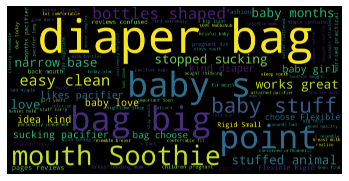
\includegraphics[width=10.5cm]{./figures/pacifier_good.png}
\caption{Wordcloud (negative) of pacifier}
\end{figure}
\begin{figure}[htbp]
\centering
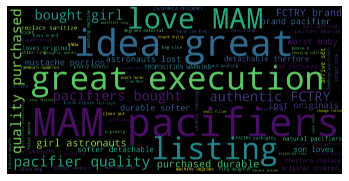
\includegraphics[width=10.5cm]{./figures/pacifier_bad.png}
\caption{Wordcloud (negative) of pacifier}
\end{figure}
\begin{figure}[htbp]
\centering
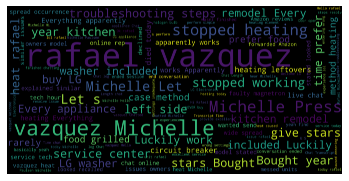
\includegraphics[width=10.5cm]{./figures/microwave_bad.png}
\caption{Wordcloud (negative) of microwave}
\end{figure}
\begin{figure}[htbp]
\centering
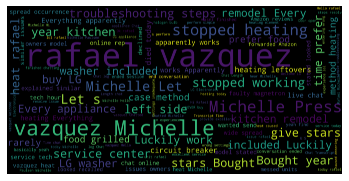
\includegraphics[width=10.5cm]{./figures/microwave_bad.png}
\caption{Wordcloud (negative) of microwave}
\end{figure}
\end{appendices}

\end{document}

%%
%% This work consists of these files mcmthesis.dtx,
%%                                   figures/ and
%%                                   code/,
%% and the derived files             mcmthesis.cls,
%%                                   mcmthesis-demo.tex,
%%                                   README,
%%                                   LICENSE,
%%                                   mcmthesis.pdf and
%%                                   mcmthesis-demo.pdf.
%%
%% End of file `mcmthesis-demo.tex'.

\end




